A maximum likelihood fit used to extract all information in this
analysis needs to be validated. The validation procedure consists of
two main tests. The first test is a fit using a data sample without
anomalous couplings. Such a test allows to identify problems with
event generation causing discrepancies in the leading lepton
\pt\ distribution. The second test is a fit using a data sample with
anomalous couplings. Such a tests demonstrates that if anomalous
couplings are present in real data that we can detect them. Both tests
are critical to validate the fitting tools, which are fairly
complicated.

In the previous analysis it was found that the leading lepton
\pt\ distribution does not allow to differentiate between different
couplings and a typical observation inconsistent with Standard Model
represents a class of possible coupling values.

Figure~\ref{fig:val_scans} shows fit results and likelihood scans for
\ww\ simulated data with and without anomalous couplings. One may
conclude that even though the fit was able to measure the couplings
close to the true values, there is large uncertainty on the angle
between the two couplings as is revealed in the shapes of the contour
plots in the likelihood scans.

\begin{figure}[tp]
  \centerline{
    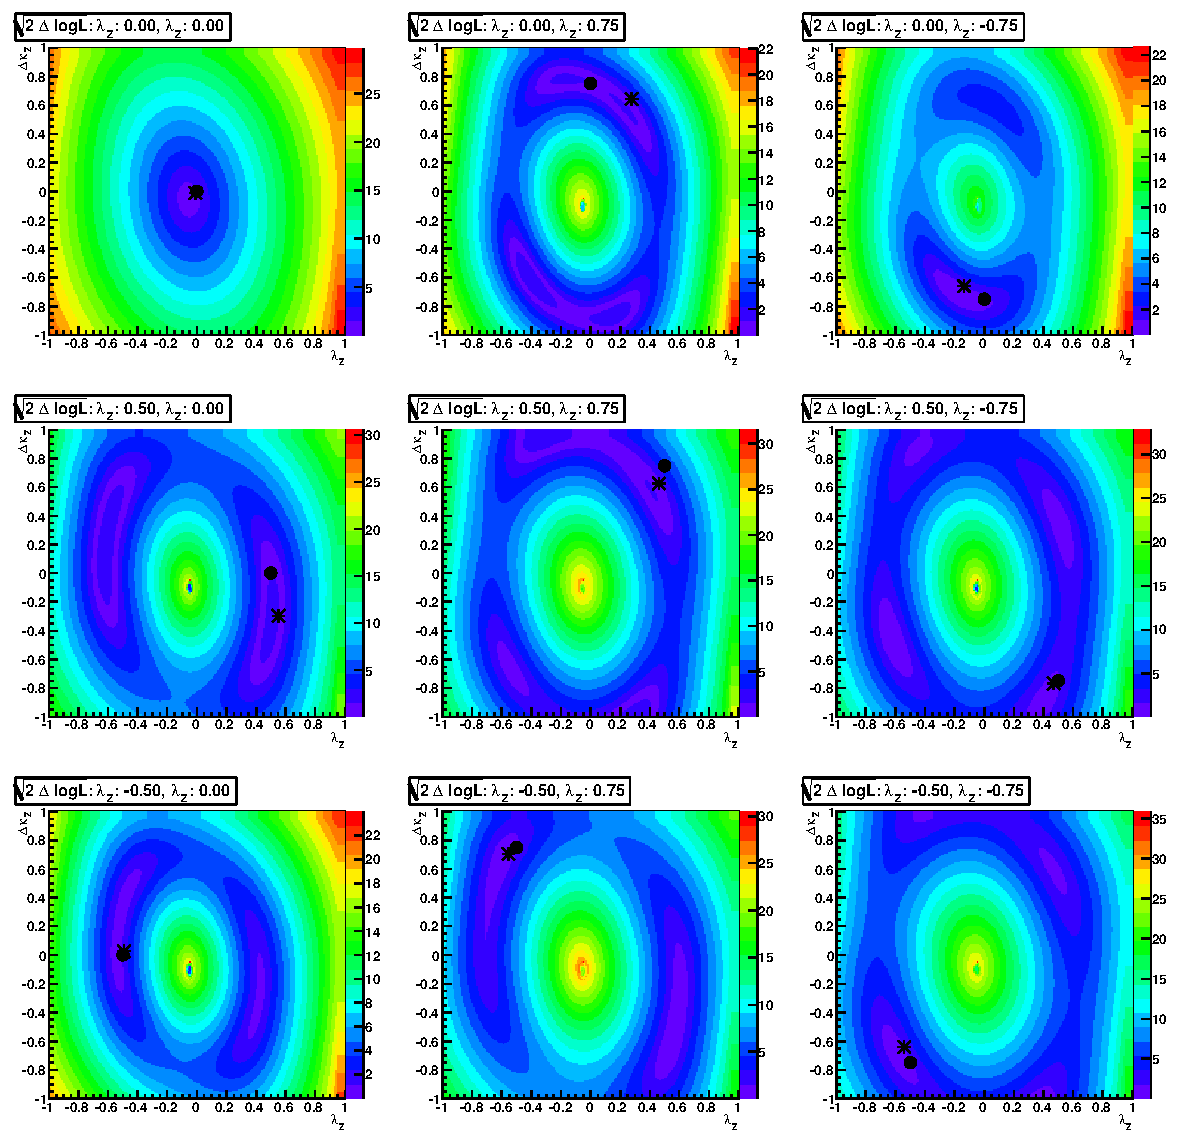
\includegraphics[width=1.0\textwidth]{figures/validation_likelihood_scans}
  }

  \caption[Likelihood scan for Signal Monte Carlo] {Likelihood scans
    for 350/pb of data excluding backgrounds. The curves
    represent the $\sqrt{2\Delta\log L}$ 1D significance of the difference between the
    likelihood with the sample's true anomalous couplings and the other
    values on the plain. The black star is the fit result when both couplings are
    allowed to float in the fit. The black point is the true value of the couplings.}
  \label{fig:val_scans}
\end{figure}

\subsection{Pseudo-experiments}
Figures~\ref{fig:fit_ww_mc_1D},
~\ref{fig:fit_ww_mc_1D_2}, \ref{fig:fit_wwATGC_mc_1D_abs} and
\ref{fig:fit_wwATGC_mc_1D_abs2} show results of the fits on \ww\ Monte
Carlo samples with and without anomalous couplings and excluding
backgrounds. If only one coupling is fitted
it is not possible to get the sign right, so only absolute
values can be measured.

Pseudo-experiments with Standard Model \ww\ Monte Carlo allows to look
for bias in the fit for the central value and to test the uncertainty
estimation. No significant deviation from zero is
found. Pseudo-experiments with aTGC \ww\ Monte Carlo samples give
consistent results with the expectations and do not find any bias in
the coupling extraction.

\begin{figure}[tp]
  \centerline{
    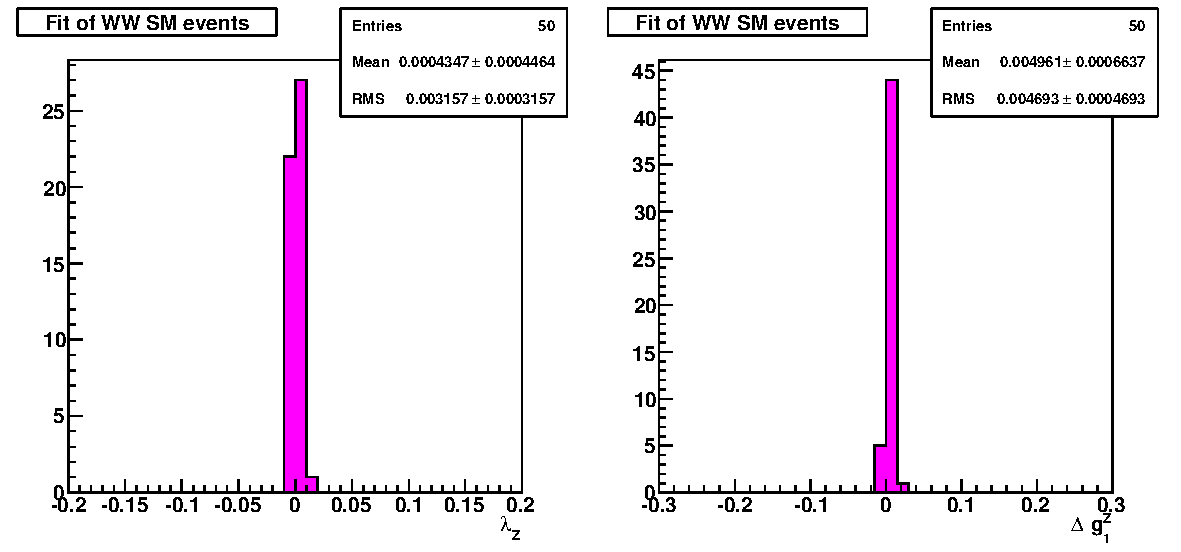
\includegraphics[width=1.0\textwidth]{figures/fit_ww_mc_1D}
  }

  \caption[1D fits to WW SM Monte Carlo] {Fit results for
  $\lambda_{Z}$ and $\Delta g^Z_1$ using 33 independent pseudo-data
  experiments made of Madgraph Standard Model \ww\ simulated
  data. Backgrounds are excluded.}

\label{fig:fit_ww_mc_1D}
\end{figure}

\begin{figure}[tp]
  \centerline{
    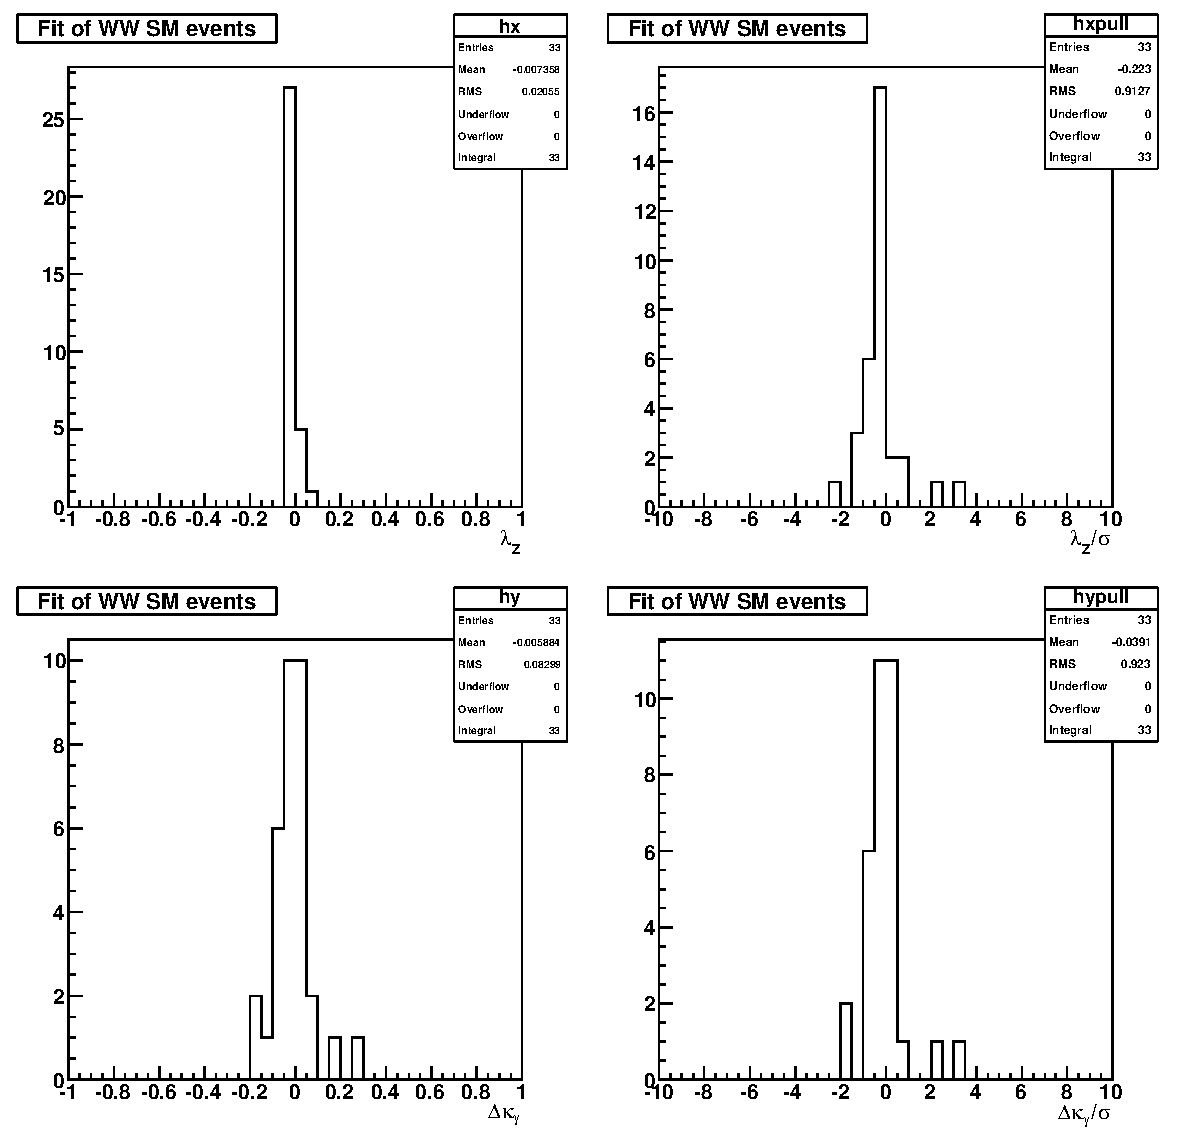
\includegraphics[width=1.0\textwidth]{figures/fit_ww_mc_1D_2}
  }

  \caption[1D fits to WW SM Monte Carlo] {Fit results for
  $\lambda_{Z}$ and $\Delta\kappa_\gamma$ using 33 independent pseudo-data
  experiments made of Madgraph Standard Model \ww\ simulated
  data. Backgrounds are excluded.}

\label{fig:fit_ww_mc_1D_2}
\end{figure}


%% \begin{figure}[tp]
%%   \centerline{
%%     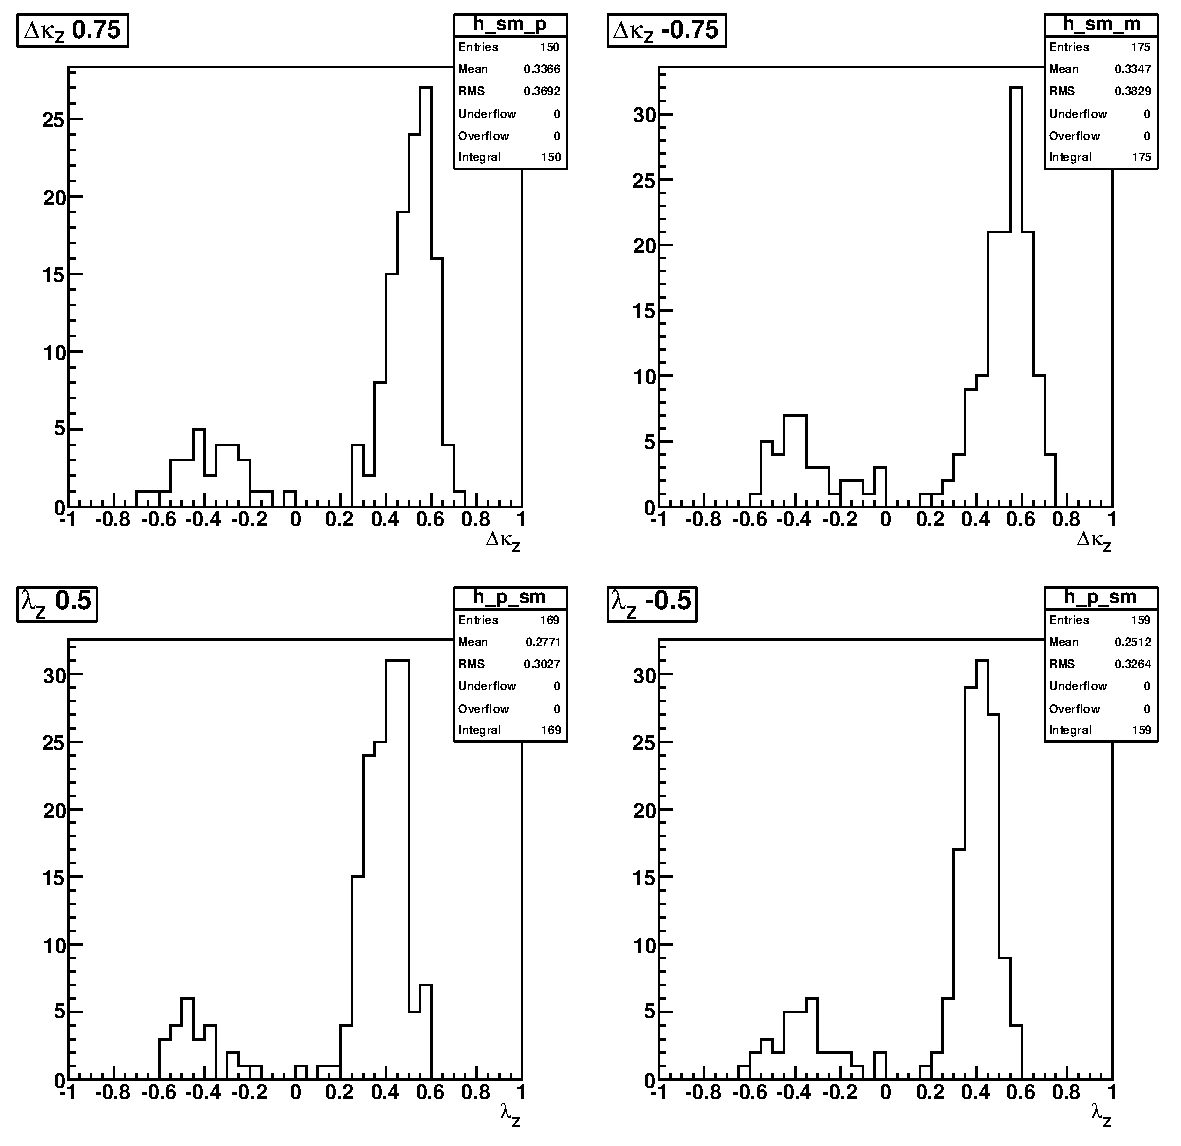
\includegraphics[width=1.0\textwidth]{figures/fit_wwATGC_mc_1D_pm}
%%   }

%%   \caption[1D fits to WW aTGC Monte Carlo] {Fits to WW Monte Carlo
%%     samples with anomalous couplings with 11 events in a sample. No
%%     background. Only one coupling is floated in the fit. Sign of the
%%     coupling cannot be determined in the fit.}
%%   \label{fig:fit_wwATGC_mc_1D_pm}
%% \end{figure}

\begin{figure}[tp]
  \centerline{
    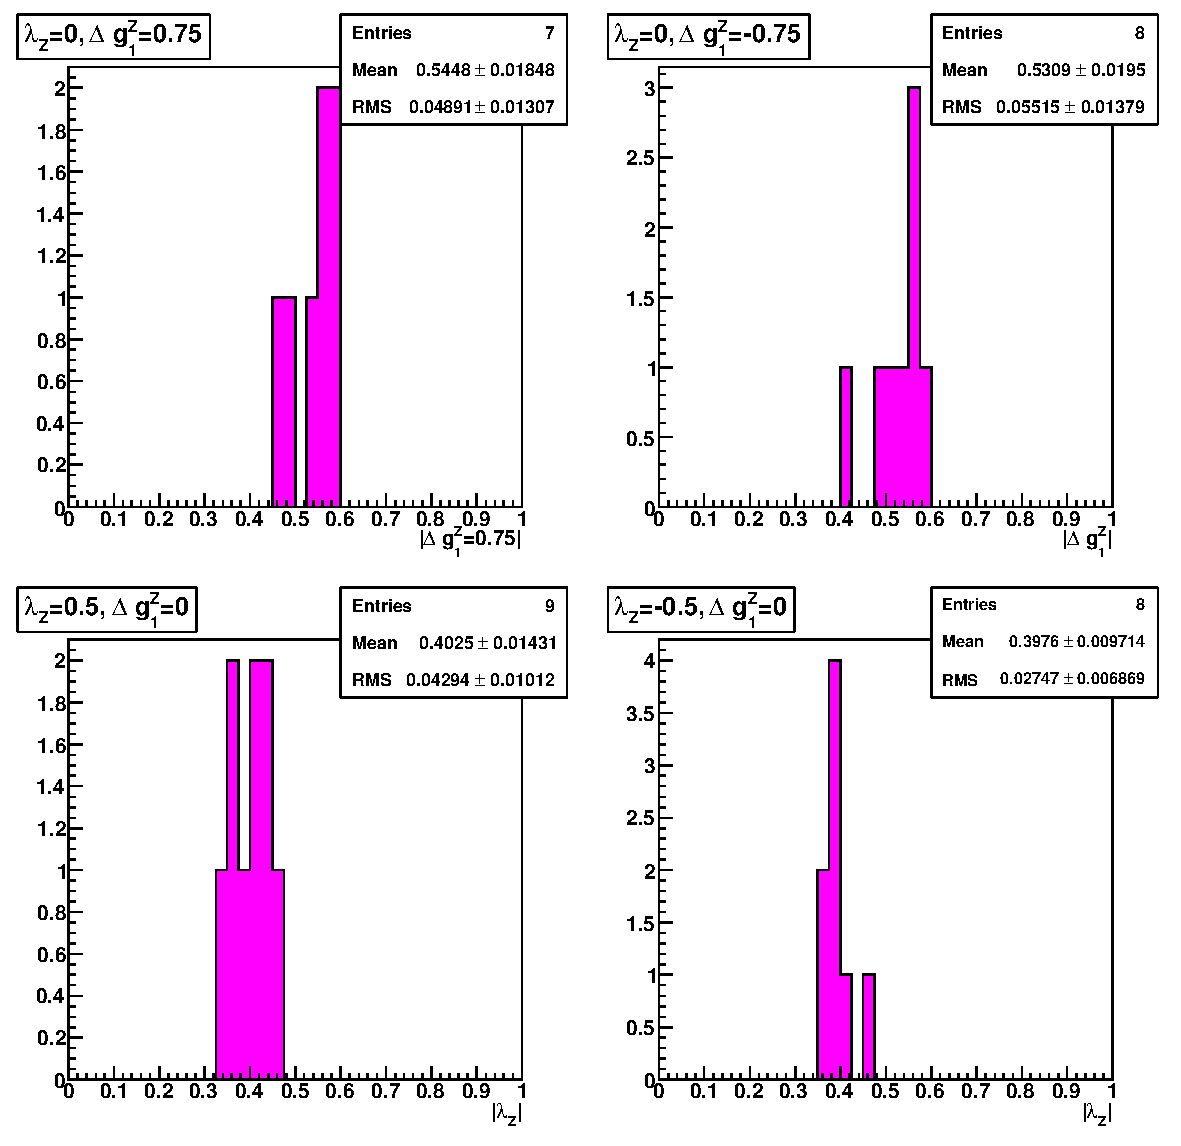
\includegraphics[width=1.0\textwidth]{figures/fit_wwATGC_mc_1D_abs}
  }

  \caption[1D fits to WW aTGC Monte Carlo] {Fits to $WW$ Monte Carlo
    samples with anomalous couplings with 100 events in each sample. Backgrounds
    are excluded. Only one coupling is allowed to float in the fit. Absolute
    values of the couplings are shown.}
  \label{fig:fit_wwATGC_mc_1D_abs}
\end{figure}

\begin{figure}[tp]
  \centerline{
    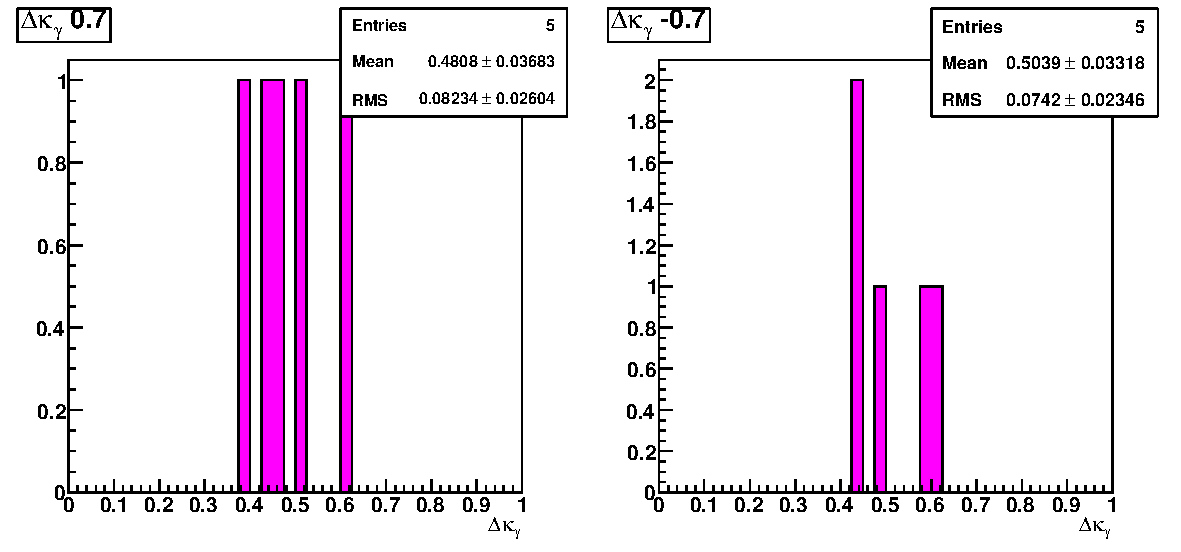
\includegraphics[width=1.0\textwidth]{figures/fit_wwATGC_mc_1D_abs2}
  }

  \caption[1D fits to WW aTGC Monte Carlo] {Fits to $WW$ Monte Carlo
    samples with anomalous couplings with 55 events in each
    sample. Backgrounds are excluded. Only one coupling is allowed to
    float in the fit. Absolute values of the couplings are
    shown.}  \label{fig:fit_wwATGC_mc_1D_abs2}
\end{figure}
